\begin{figure}[H]
\scalebox{0.5}{%
    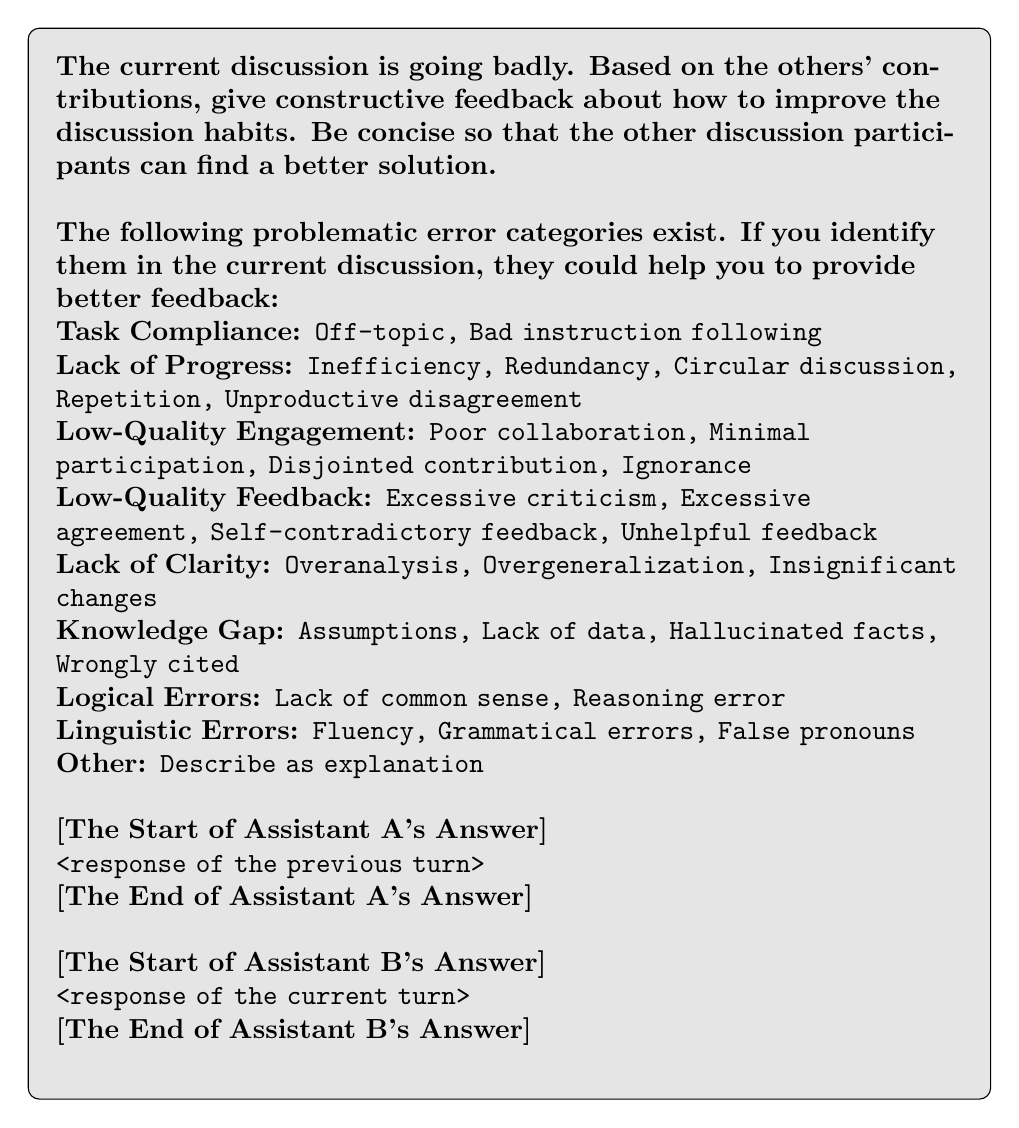
\begin{tikzpicture}
    \node [draw, rectangle, rounded corners, fill=gray!20, text width=0.95\textwidth, inner sep=10pt] (block) {
        \begin{minipage}{\textwidth}
        \textbf{The current discussion is going badly. Based on the others' contributions, give constructive feedback about how to improve the discussion habits. Be concise so that the other discussion participants can find a better solution.}\\

        \textbf{The following problematic error categories exist. If you identify them in the current discussion, they could help you to provide better feedback:}\\
        \textbf{Task Compliance:} \texttt{Off-topic, Bad instruction following}\\
        \textbf{Lack of Progress:} \texttt{Inefficiency, Redundancy, Circular discussion, Repetition, Unproductive disagreement}\\
        \textbf{Low-Quality Engagement:} \texttt{Poor collaboration, Minimal participation, Disjointed contribution, Ignorance}\\
        \textbf{Low-Quality Feedback:} \texttt{Excessive criticism, Excessive agreement, Self-contradictory feedback, Unhelpful feedback}\\
        \textbf{Lack of Clarity:} \texttt{Overanalysis, Overgeneralization, Insignificant changes}\\
        \textbf{Knowledge Gap:} \texttt{Assumptions, Lack of data, Hallucinated facts, Wrongly cited}\\
        \textbf{Logical Errors:} \texttt{Lack of common sense, Reasoning error}\\
        \textbf{Linguistic Errors:} \texttt{Fluency, Grammatical errors, False pronouns}\\
        \textbf{Other:} \texttt{Describe as explanation}\\

        \textbf{[The Start of Assistant A's Answer]} \\
        \texttt{<response of the previous turn>}\\
        \textbf{[The End of Assistant A's Answer]} \\

        \textbf{[The Start of Assistant B's Answer]} \\
        \texttt{<response of the current turn>}\\
        \textbf{[The End of Assistant B's Answer]} \\
        \end{minipage}
    };
    \end{tikzpicture}
}
\caption{Prompt for the policy feedback agent.}
\end{figure}
